 \documentclass[style=upen, size=14pt]{powerdot}
\definecolor{arany}{RGB}{255,242,0}
\hypersetup{backref=page}
\hypersetup{
    colorlinks=true,
    linkcolor=cyan,
    filecolor=magenta,      
    urlcolor=cyan}
\usepackage{graphicx}
\usepackage{amsmath}
\DeclareMathOperator*{\argmax}{argmax}
\DeclareMathOperator*{\argmin}{argmin}
\usepackage{amssymb}
\usepackage{stmaryrd}
\usepackage[latin2]{inputenc}
%\usepackage[magyar]{babel}
%\usepackage{euler}
\usepackage{tikz}
\usepackage{tikz-qtree}
\tikzset{every tree node/.style={align=center,anchor=north}}
%\usepackage{tabularx}
%\usepackage{threeparttable}
%\usepackage{color}
%\selectlanguage{english}
%\frenchspacing
\newcommand{\nd}{\noindent}
\newcommand{\Val}{\mathop{\mathit{Val}}}
\newcommand{\gold}{\color{arany}}
%\usepackage{tikz}
%\usepackage{tikz-qtree}
\newcommand{\qed}{\hfill\mbox{\raggedright \rule{.1in}{.1in}}}
\def\es{\mathbin\land}
\newtheorem{defi}{Definition}
\newtheorem{axioma}{Axióma}
\newtheorem{tetel}{Theorem}
\newtheorem{prop}{Proposition}
\newtheorem{lemma}{Lemma}
\begin{document}
\title{Natural Language Processing\\~~\\Lecture 1\\Introduction}
\author{Andr�s Simonyi, ELTE, Department of AI}

\date{2021}
\maketitle

\begin{slide}{Course textbooks}
  \pause
  \begin{itemize}
  \item  Dan Jurafsky and James H. Martin,\\
    \emph{Speech and Language Processing} 3rd ed.\\
    Draft available at \href{https://web.stanford.edu/~jurafsky/slp3}{https://web.stanford.edu/$\sim$jurafsky/slp3}.\pause
  \item Jacon Eisenstein,\\
    \emph{Natural Language Processing}.\\
    Available at
    \href{https://github.com/jacobeisenstein/gt-nlp-class}{https://github.com/jacobeisenstein/gt-nlp-class}.
  \end{itemize}\pause
  These slides are in large part based on the first, "Introduction" chapter of
  the Eisenstein book.
\end{slide}

\begin{slide}[toc=What is NLP?]{What is Natural Language Processing?}
  {\gold NLP} is an interdisciplinary field concerned with making natural
  languages accessible to computers.\pause
  \begin{itemize}
  \item {\gold Natural language} in this context means the ordinary
    languages humans use to communicate in speech or writing, e.g., English,
    Chinese, Spanish etc.\pause
  \item Being able to {\gold access} natural language covers a wide range
    of capabilities, with important areas being\pause
    \begin{itemize}
    \item {\gold communication}: the ability to accept input and produce
      output in natural language;\pause
    \item {\gold understanding}: being able to access and utilize the
      informational and emotional content;\pause
    \item {\gold linguistic assistance}: the ability to help humans to
      express themselves linguistically.
    \end{itemize}
  \end{itemize}
\end{slide}

\section{Related fields}

\begin{slide}[toc=CompLing]{Computational linguistics}
  The scientific study of language using computational methods.\pause
  \begin{itemize}
  \item Perhaps the closest field to NLP, but with a different focus: NLP is
    \emph{not} concerned with theoretical insights into natural languages
    \emph{per se} but only with the design and analysis of methods useful for
    computational language processing.\pause
  \item Instead of direct implementations of theoretical ideas, it often provides
    \emph{architectural inspiration} for NLP systems.
  \end{itemize}
\end{slide}

\begin{slide}[toc=AI]{Artificial intelligence (AI)}
  There is obviously a large overlap between the NLP objective and AI's goal of
  building intelligent systems:\pause
    \begin{itemize}
    \item language use is strongly interdependent with the conceptual,
      representational and reasoning capabilities required for being
      intelligent,\pause
    \item in practice, large-scale knowledge acquisition is also impossible without the
      ability to extract information from natural language input.
    \end{itemize}\pause
    The above characteristics make especially the AI subfield {\gold 
      Knowledge Representation and Reasoning} very relevant for NLP.
\end{slide}

\begin{slide}[toc=Machine learning]{Machine learning}
  Modern NLP relies on machine learning techniques to a huge extent, in fact, in
  recent years the linguistic applications of general ML methods have dominated
  the area.\pause
  \begin{itemize}
  \item Mostly supervised or semi-supervised methods are utilized, but the use
    of reinforcement learning is also increasing.\pause
  \item Texts are sequences of discrete symbols, so ML models capable of dealing
    with this type of input (and output in case of generation) are needed.
  \end{itemize}
\end{slide}


\begin{slide}[toc=Speech processing]{Speech processing}
  The processing and generation of acoustic speech signals is traditionally not
  considered part of NLP, which is concerned primarily with \emph{texts}, but is
  obviusly closely related:\pause
    
  \begin{itemize}
  \item Speech2text provides input for NLP applications,\pause
  \item NLP apps provide input for speech synthesis;\pause
  \item Both processing and synthesizing speech requires linguistic knowledge
    that is also relevant for NLP: especially \emph{language modeling} has a
    central role in both areas.
  \end{itemize}
\end{slide}

% \begin{slide}[toc=]{Related fields cont.}
%   \begin{itemize}
%   \item {\gold Computer science}:
%   \item {\gold Ethics}:
%   \end{itemize}
% \end{slide}

\section{Applications}

\begin{slide}[toc=Examples]{Application examples}
  \begin{itemize}
  \item {\gold machine translation},\pause
  \item {\gold document retrieval}: retrieving free-text documents matching a
    user query,\pause
  \item {\gold question answering}, e.g., smart phone assistants'
    ability to answer questions,\pause
  \item {\gold text classification}, e.g. detecting e-mail spam,\pause
  \item {\gold chatbots}, e.g., a chatbot for buying a train ticket,\pause
  \item {\gold spell checking} and {\gold grammar checking},\pause
  \item {\gold auto-completion} for free-text input,\pause
  \item {\gold document summarization},\pause
  \item {\gold text generation} from structured data (from stock exchange news
    to error messages).
  \end{itemize}
\end{slide}

\section{Central themes}

\begin{slide}[toc=Pipeline]{Pipeline vs end-to-end architectures}
  An influential view of NLP considers its core task to provide a {\gold
    pipeline of modules} that successively produce general-purpose linguistic
  analyses, each module building on the outputs of the previous ones: \bigskip

  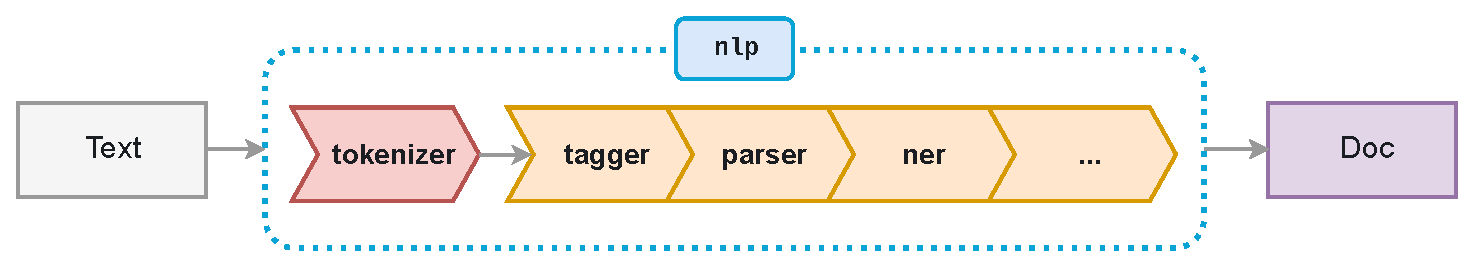
\includegraphics[width=1.05\textwidth]{figures/pipeline.eps}
  
  \footnotesize{(Figure from the
    \href{https://spacy.io/usage/processing-pipelines}{documentation of the
      spaCy NLP library}.)}\bigskip\pause
  
  \normalsize Specialized NLP applications are then built as relatively simple
  additions on top of elements of this universal pipeline.
\end{slide}

\begin{slide}[toc=End-to-end]{Pipeline vs end-to-end cont.}
  The opposite view concentrates on building NLP applications as {\gold
    end-to-end} machine learning models that learn to transform the raw input to
  the required output without specialized linguistic analyzer modules.\pause

  \bigskip
  
  State-of-the art NLP applications frequently fall in between these two
  extremes: they use some universal analyzer modules, e.g., for word
  segmentation or stemming, and also rely on ML models that skip some of the
  traditional pipeline steps to produce the required output.
\end{slide}

\begin{slide}{Transfer learning}
  An interesting, relatively recent, development is the appearance of neural
  models that are end-to-end pretrained on unsupervised tasks on very large text
  collections, and can act as a replacement for the traditional processing
  pipelines:\pause
  \begin{itemize}
  \item Specialized models can be built by adding a few very shallow layers to
    the architecture but keeping the pretrained weights perhaps with a bit of
    fine-tuning.\pause
  \item It seems that some components of traditional pipeline have neural
    analogues in these models: certain layers seem to learn (more) morphology,
    others semantics etc.\pause
  \end{itemize}
\end{slide}

\begin{slide}{Learning and search}
  A large number of supervised NLP tasks which we will encounter can be
  formulated as an optimization problem of the form
  $$\hat y = \argmax_{y\in Y(x)}\Psi_\theta(x, y)$$\pause
  where
  \begin{itemize}
  \item $x\in X$ and $Y(x)$ are the task's input and potential outputs,\pause
  \item $\Psi_\theta: X\times Y \rightarrow \mathbb R$ is a scoring function or
    model that assigns scores to $\langle x, y \rangle$ input-output pairs and
    is parametrized by a $\theta$ vector, \pause and
  \item $\hat y$ is the predicted output.
  \end{itemize}
\end{slide}

\begin{slide}[toc=]{Learning and search cont.}
  For instance,
  \begin{itemize}
  \item  $X$ could contain movie reviews and $Y$ the sentiment labels
  \textsc{Positive}, \textsc{Negative} and \textsc{Neutral}, and $\Psi_\theta$
  could be a function assigning probabilities to the possible sentiment labelings
  of the reviews.\pause
\item Also, $X$ could be the set of German texts and $Y$ their potential English
  translations, with $\Psi_\theta$ assigning translation quality scores to the
  candidates.\pause
  \end{itemize}
\end{slide}

\begin{slide}[toc=]{Learning and search cont.}
  This formulation makes it possible to factorize the problem into two
  optimization subproblems solved by two distinct modules:\pause
  \begin{itemize}
  \item {\gold Learning:} Finding the optimal $\theta$ parameters. This is
    typically done by optimizing $\theta$ on a large supervised data set
    $\{\langle x_i, y_i \rangle\}_{i=1}^N$ using numerical optimization methods.\pause
  \item {\gold Search:} Finding the best scoring $y$ for a specific $x$, i.e.,
    computing the value of the $\argmax$ in the formula. Since the search space
    $Y(x)$ is often large because the potential $y$s have a complex structure
    (think, e.g., of a parse tree), this problem frequently requires
    combinatorial optimization.
  \end{itemize}
\end{slide}

\begin{slide}[toc=Relational semantics]{Semantic perspectives: relational}
  Consider the utterance

  \bigskip
  \emph{My uncle's bought a cat. He's perhaps the most obnoxious animal I've ever met.}
  \pause
  \bigskip

  How do we know that ``animal'' refers to the mentioned cat? One factor is
  that we know that \emph{cat} is a subcategory of \emph{animal}: they are
  connected by the \textsc{is\_a} relationship.\pause

  \bigskip

  The {\gold relational perspective} concentrates on these semantic/conceptual
  links between the senses of expressions, which together constitute semantic
  networks:
\end{slide}

\begin{slide}[toc=]{Semantic perspectives: relational}
  
\includegraphics[width=0.7\textwidth]{figures/semantic_net.eps}

 % \bigskip
  
  \scriptsize{(A semantic network fragment. Figure from
    \href{https://en.wikipedia.org/wiki/Semantic_network}{Wikipedia: Semantic
      Networks.})}

  \bigskip \normalsize Lexical semantic ontologies like WordNet and FrameNet are
  attempts to enumerate the semantic relations between a large number of word
  senses.
\end{slide}

\begin{slide}[toc=Compositionality]{Semantic perspectives: compositionality}
  The relational view sees meanings as atomic nodes in a network. The {\gold
    compositional perspective}, in contrast, analyzes an expression's meaning
  according to its internal composition.\pause

  \bigskip
  
  E.g., the decomposition \bigskip

  \emph{un$\vert$bear$\vert$able$\vert$s}\pause

  \bigskip allows us to see the meaning of \emph{unbearables} as being composed of
  the meanings of its parts \emph{un}, \emph{bear}, \emph{able} and \emph{s}.
\end{slide}

\begin{slide}[toc=]{Semantic perspectives: compositionality}
  The principle of compositionality:\pause

  \bigskip
  
  \emph{The meaning of a complex expression
    is determined by the meanings of its constituent expressions and the rules
    used to combine them.}
  \footnote{\href{https://en.wikipedia.org/wiki/Principle_of_compositionality}{Wikipedia:
      Principle of Compositionality.}}\pause

  \bigskip
  
  The principle can be applied to larger linguistic units than words: sentences
  or even paragraphs etc. One (traditional) approach is to represent meanings
  with logical formulas and associate syntactic syntactic rules of combination
  with semantic/logical  ones:
  
\end{slide}


\begin{slide}[toc=]{Semantic perspectives: compositionality}
  \begin{center}
    \Tree 
    [.{\textit{John visits Julie} (S)}
        [.{\textit{John} (NP)} ]
        [.{\textit{visits Julie} (VP)} 
             [.{\textit{visits} (VT)} ] 
             [.{\textit{Julie} (NP)} ] ] ]
  \end{center}\pause
  \begin{center}
    \Tree 
    [.{\textsc{visits}(\textsc{john},\textsc{julie})}
        [.{\textsc{john}} ]
        [.{$\lambda x.$\textsc{visits}$(x,$\textsc{julie}$)$} 
             [.{$\lambda y.\lambda x.$\textsc{visits}$(x, y)$} ] 
             [.{\textsc{julie}} ] ] ]
  \end{center}
\end{slide}

\begin{slide}[toc=Distributional]{Semantic perspectives: distributional}
  What does ``bardiwac'' mean?\footnote{The example is from Stefan Evert's
    \href{https://esslli2016.unibz.it/wp-content/uploads/2015/10/dsm_tutorial_part1.slides.pdf}{Distributional
      semantics slides}.}\pause

  \begin{itemize}
  \item He handed her a glass of {\gold bardiwac}.\pause
  \item Beef dishes are made to complement the {\gold bardiwacs}.\pause
  \item The drinks were delicious: blood-red {\gold bardiwac} as well as light,
    sweet Rhenish.\pause
  \item Nigel's face flushed from too much {\gold bardiwac}.\pause
  \item Malbec is one of the lesser-known {\gold bardiwac} grapes.\pause
  \item I dined off bread, cheese and this excellent {\gold bardiwac}.\pause
  \end{itemize}
  
  $\Rightarrow$ Bardiwac is a heavy red alcoholic beverage made from
  grapes.
\end{slide}

\begin{slide}[toc=]{Semantic perspectives: distributional}
  Even if we don't know the place of ``bardiwac'' in a semantic network nor the
  meanings of its parts, the \emph{contexts} in which it occurs provide a large
  amount of information about it's meaning.\pause

  \bigskip

  The distributional hypothesis:\pause
  \begin{itemize}
  \item ``You shall know a word by the company it keeps.''
    \footnote{J.R. Firth, \emph{Papers in Linguistics 1934--1951 (1957).}}\pause
  \item ``Linguistic items with similar distributions have similar meanings.''
    \footnote{\href{https://en.wikipedia.org/wiki/Distributional_semantics}{Wikipedia:
        Distributional semantics.}}
  \end{itemize}
\end{slide}

\begin{slide}[toc=]{Semantic perspectives: distributional}
  An important practical advantage of the distributional approach to meaning is
  that it makes it possible to learn the semantics of words automatically from
  large but unlabeled text collections, no expert knowledge and annotations are
  needed.\pause
  
  \bigskip

  The approach is not without limitations, of course:\pause
  \begin{itemize}
  \item has problems with rare words; and\pause
  \item learns the similarities without providing any explanation \emph{why}
    these distributions are similar.
  \end{itemize}
\end{slide}

\end{document}


%%% Local Variables:
%%% mode: latex
%%% TeX-master: t
%%% End:
